% siminos/reversal/latt1d.tex      pdflatex LC21; bibtex LC21
% temporary:  siminos/spatiotemp/chapter/LC21latt1d.tex
% $Author: predrag $ $Date: 2021-12-24 01:25:20 -0500 (Fri, 24 Dec 2021) $

% Predrag 2021-08-08: shared with siminos/reversal/LC21.tex

%%%%%%%%%%%%%%%%%%%%%%%%%%%%%%%%%%%%%%%%%%%%%%%%%%%%%%%%%%%%%%%
\section{Translations and reflections} %{Dihedral group}
\label{s:latt1d}
                                         \toCB

Though this exposition is nominally about `evolution in time', `time' is
such a loaded notion, a straightjacket hard to escape, that it is best to
forget about `time' for time being, and think instead like a
crystallographer, about lattices and the space groups that describe their
symmetries.

Of necessity, there many group-theoretic notions a crystallographer must
juggle (see \toChaosBook{section.11.2}{sect.~11.2}), but only a few key
things to understand:
\begin{itemize}
  \item[(i)]
For a 1\dmn\ lattice, there are only two kinds of qualitatively different
symmetry transformations,
translations \refeq{DinftyClassShift}
and
  \item[(ii)]
reflections \refeq{shiftRefl} which reverse the direction of translation.
  \item[(iii)]
There are two kinds of reflections \refeq{DinftyClassRefl}, across a lattice site,
and across a mid-point between lattice sites, \reffig{fig:HL1dLattRefl}.
  \item[(iv)]
Even though both the lattice \lattice\ and its space group $\Group$ are
infinite, \emph{orbits} of {\lattstate}s are finite and described
by finite cyclic and dihedral groups, \reffig{fig:1dLatStatC_5}.
\end{itemize}
Should the reader find symmetries of infinite lattices too obstruse:
to understand all that one needs to know about translations  and
reflections, it suffices to understand the symmetries of a
triangle and a square, \reffig{fig:D3D4}.

%%%%%%%%%%%%%%%%%%%%%%%%%%%%%%%%%%%%%%%%%%%%%%%%%%%%%%%%%%%%%%%%%%%%%%%%%%
\subsection{Symmetries of 1\dmn\ lattices, sublattices}
\label{s:1dLatt}

A space group $\Group$ is the set of all translations and rotations that
puts a crystallographic structure \lattice\ in coincidence with itself.
To make the exposition as simple as possible, here we focus on 1\dmn\
crystals, with sites labeled by integer lattice $ \lattice=\integers$.
Their space groups crystallographers\rf{Dresselhaus07} call \emph{line
groups}.
%
There are only two \HREF{https://en.wikipedia.org/wiki/Line_group}
{1\dmn\ space groups}  $\Group$: $p1$, or the \emph{infinite cyclic
group}  \Cn{\infty} of all lattice translations,
and
$p1m$, the \emph{infinite dihedral group} $\Dn{\infty}$  of all
translations and reflections\rf{KiLePa03},
\beq
  \Dn{\infty} = \{
\cdots, \shift_{-2},\Refl_{-2}, \shift_{-1},\Refl_{-1},
        1,\Refl,
        \shift_{1},\Refl_{1}, \shift_{2},\Refl_{2}, \cdots
             \}
\,.
\ee{LC21D_infty}
A half of the elements are translations (`shifts'; for finite period
lattices, `rotations').
$\shift_{0}=1$ denotes the identity,
and
the
$\shift_{1}=\shift$, $\shift_{2}=\shift^2$, $\cdots$,
$\shift_{k}=\shift^k$, $\cdots$,
denote translations by $1,2,\cdots,k,\cdots$ lattice points. They form
the \emph{infinite cyclic group}
\beq
\Cn{\infty}
    =       \{
\cdots, \shift_{-2}, \shift_{-1},
        1,
        \shift_{1}, \shift_{2}, \shift_{3}, \cdots
             \}
\,,
\label{C_infty}
\eeq
a subgroup of $\Dn{\infty}$,
in crystallography called the translation group.

The other half of elements are reflections $\Refl_{k}^2=1$
(`inversions', `time reversals', `flips'), defined by first translating
by $k$ steps, and then reflecting, resulting in a `translate-reflect'
operation
\beq
\Refl_{k}=\Refl\shift_k
\,.
\ee{Refl_k}

The defining property of translate \& reflect groups
(`dihedral' groups, `flip systems'\rf{KiLePa03}) is that
any reflection reverses the direction of the translation
\beq
\Refl_{k}\shift = \shift^{-1}\Refl_{k}
\,.
\ee{shiftRefl}
%
The group multiplication (or `Cayley') table for successive group actions
$\LieEl_i\LieEl_j$ follows:
\beq
\begin{tabular}{c|cc}
%\Dn{\infty} &\shift_j        &\Refl_j\\\hline
            &$\shift_j$        &$\Refl_j$\\\hline
$\shift_i$  &$\shift_{i+j}$     &$\Refl_{j-i}$\\
$\Refl_i$   &$\Refl_{i+j}$     &$\shift_{j-i}$
\end{tabular}
\,.
\ee{eq:DinftyMultTab}
Multiplication either adds up translations,
or shifts and then reverses their direction.
The order in which the elements $\LieEl_i\LieEl_j$ act is right to left,
\ie, a group element acts on the expression to its right.

A crystallographer organizes the \emph{subgroups} of a space group
$\Group$ by means of \emph{Bravais lattices} $\lattice_\mathbf{a}$,
sublattices of the lattice $\integers$, each defined here by a 1\dmn\
\emph{Bravais cell} of \emph{period} \cl{}, given by a lattice vector
$\mathbf{a}$ of integer length \cl{},
\beq
\lattice_\mathbf{a} = \{j \mathbf{a} \,|\, j \in \integers\}
\,,
\ee{1DBravLatt}
with the lattice generated by the infinite translation group of all
discrete translations replaced by
\[
  \shift_{j}\to\shift_{j\mathbf{a}}
\]
multiples of $\mathbf{a}$, resulting in
\beq
H_{\mathbf{a}} = \{ \cdots, \shift_{-2 \mathbf{a}}, \shift_{-\mathbf{a}},
1, \shift_{\mathbf{a}}, \shift_{2 \mathbf{a}}, \cdots\}
\,,
\ee{H(n)subgroup}
infinite translation subgroup of the infinite translation group
$\Cn{\infty}$. You can visualize a {\lattstate} invariant under subgroup
$H_{\mathbf{a}}$ as a tiling of the lattice $\integers$ by a generic
{\lattstate} over tile of length \cl{}.
% , \reffig{fig:1dLatStatC_5}\,(1).

%The infinite translation group $H_{\mathbf{a}}$ is a  subgroup of
%$\Cn{\infty}$, itself a subgroup
%% $\Cn{\infty}\subset\Dn{\infty}$
%of the system symmetry $\Group=\Dn{\infty}$.
Another family of subgroups of
$\Dn{\infty}$ is obtained
by substituting elements of $\Dn{\infty}$ \refeq{LC21D_infty} by
\[
  \shift_{j}\to\shift_{j\mathbf{a}}
\,,\qquad
    \Refl\to \Refl_{k}
  \quad
     0\leq{k}<\cl{}
\,,
\]
resulting in $\cl{}$ infinite dihedral groups
\beq
H_{\mathbf{a},k} = \{
\cdots, \shift_{-2 \mathbf{a}}, \Refl_{k}\shift_{-2 \mathbf{a}},
        \shift_{-\mathbf{a}}, \Refl_{k}\shift_{-\mathbf{a}},
        1,                    \Refl_{k},
        \shift_{\mathbf{a}},  \Refl_{k}\shift_{\mathbf{a}},
        \shift_{2\mathbf{a}},\Refl_{k}\shift_{2\mathbf{a}}, \cdots
             \}
\,,
\ee{H(n,k)subgroup}
each given by a {Bravais cell} of period \cl{}, with reflection
across a symmetry point shifted $k$ half-steps, see
\refeq{1dLattRefl1}.


%%%%%%%%%%%%%%%%%%%%%%%%%%%%%%%%%%%%%%%%%%%%%%%%%%%%%%%%%%%%%%%%%%%%%%%%%%
\subsection{Classes}
\label{s:1dLattClass}

    \begin{quote}
Definition:
{\em A class is the set of elements left
invariant by conjugation with all elements $\LieEl$ of the group \Group,
where an element $b$ is \emph{conjugate} to element $a$ {if}

}
\beq
b = \LieEl\,a\,\LieEl^{-1}
\,.
\ee{conjugate}
    \end{quote}



By \refeq{shiftRefl}, a conjugation by any reflection reverses the
direction of translation
\beq
   \Refl_i\shift_j\Refl_{-i} =  \shift_{-j}
\,,
\ee{DinftyInversion}
so every translation pairs up with the equal counter-translation to form
\bea
\mbox{identity class }
    &&\qquad
\{1\}
    \,,\quad\qquad\;
j=0
    \label{DinftyClassId}\\
\mbox{translation classes }
    &&\qquad
\{\shift_j,\shift_{-j}\}
    \,,\quad
j=1,2,3,\cdots
\,.
\label{DinftyClassShift}
\eea
The $\shift_{0}=1$ commutes with all group elements, and is thus always a
class by itself.

From the multiplication table \refeq{eq:DinftyMultTab} it
follows that a conjugate of a reflection
\beq
\shift_i\,\Refl_j\shift_i^{-1}      % = \Refl_{i+j}\shift_{-i}
= \Refl_{j-2i}
\,, \quad
\Refl_i\Refl_{j}\Refl_i^{-1}  % = \shift_{i-j}\Refl_i
= \Refl_{2i-j}
\,.
\ee{D_nConj}
is a reflection related to it by a ${2i}$ translation.
Hence the even subscript reflections belong to one class, and the odd
subscript reflections to the other:
\bea
\mbox{even}
    &&\quad
\{\Refl_{2m}\}
\,,\qquad
m\in\integers
    \continue
\mbox{odd}
    &&\quad
\{\Refl_{2m+1}\}
\,.
\label{DinftyClassRefl}
\eea
By \refeq{D_nConj} $r H_{\cl{},k} r^{-1} = H_{\cl{},k-2}$, so for odd
\cl{}, there are $\cl{}$ Bravais sublattices in the class, and
for even \cl{}, $H_{\cl{},k}$ separate into 2 classes
\refeq{DinftyClassRefl},
\bea
\mbox{even}
    &&\quad
\{H_{2m,2j}\}
\,,\qquad
0\leq j<\cl{}/2
    \continue
\mbox{odd}
    &&\quad
\{H_{2m,2j+1}\}
\,,
\label{H(n,k)class}
\eea
each containing  $m$ Bravais sublattices.

%%%%%%%%%%%%%%%%%%%%%%%%%%%%%%%%%%%%%%%%%%%%%%%%%%%%%%%%%%%%%%%%%%%%%%%%%%
\subsection{Reflections}
\label{s:1dLattRefl}

What's the difference between an `odd' and an `even' reflection?
Every {element} in a class is equivalent to
any other of its {element}s.
% , up to a symmetry-group coordinate frame transformation.
So, to understand what everybody in a given class does, it suffices to
work out what a single representative does:
it suffices to analyse the $H_{\cl{},0}$ and $H_{\cl{},1}$
to account for all $H_{\cl{},k}$.

So far,
we have only discussed the abstract structure of the space group
$\Dn{\infty}$  and its subgroups. But the difference between an `odd' and
an `even' is easiest to grasp by working out the action of $\Refl_k$ on a
{\lattstate}.

%%%%%%%%%%%%%%%%%%%%%%%%%%%%%%%%%%%%%%%%%%%%%%%%%%%%%%%%%%%%%%%%%%
\begin{figure} \begin{center}
  \begin{minipage}[b]{0.40\textwidth}\begin{center}
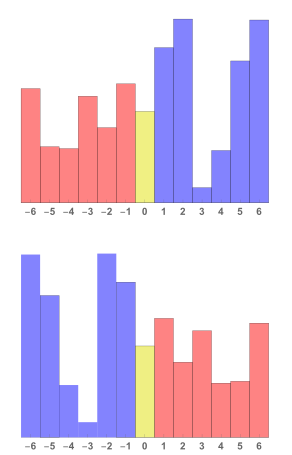
\includegraphics[width=\textwidth]{HL1dLattRefl0}
  \\ (even)
  \end{center}\end{minipage}
\qquad
  \begin{minipage}[b]{0.40\textwidth}\begin{center}
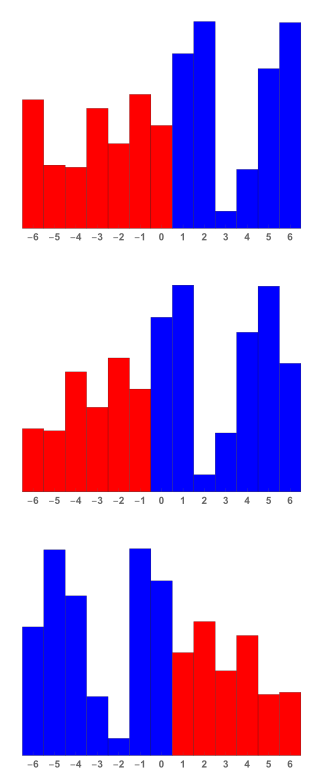
\includegraphics[width=\textwidth]{HL1dLattRefl1}
  \\ (odd)
  \end{center} \end{minipage}
  \end{center}
  \caption{\label{fig:HL1dLattRefl}
(Color online)~~~
There are two classes %\refeq{DinftyClassRefl}
of {\lattstate} reflections,
even \refeq{1dLattRefl0} and odd \refeq{1dLattRefl1}.
% :
% even, across a lattice site, and odd, across the mid-point between
% a pair of adjacent lattice sites.
    (Even)
reflection $\Refl$ exchanges (blue
$\ssp_j$) $\leftrightarrow$  (red $\ssp_{-j}$) %, $j>0$,
while leaving the yellow
field $\sitebox{\ssp_0}$ at lattice site ${0}$ fixed.
    (Odd)
reflection $\Refl_1=\Refl\shift$ swaps the
`blues' and the `reds' by a lattice
translation $\Xx\to\shift\Xx$, followed by a reflection $\Refl$. The
result is a reflection across the midpoint of the [01] interval,  marked
`|'.
See \reffig{LC21FieldConfig}\,(b) for the notation.
% Horizontal: lattice sites $j\in\integers$. Vertical: lattice site
% fields $\ssp_j$, labeled by their values before the reflection.
}
\end{figure}
%%%%%%%%%%%%%%%%%%%%%%%%%%%%%%%%%%%%%%%%%%%%%%%%%%%%%%%%%%%%%%%


\paragraph{Even class.}
Take $\Refl=\Refl_0$ as a representative of all even reflections
$\Refl_{2m}$,  and act on a {\lattstate} \refeq{1dLattStat}:
\bea
\Xx &=&
\cdots {\ssp}_{-3} {\ssp}_{-2}\,{\ssp}_{-1}\,
       {\ssp}_0\,
      {\ssp}_{1} {\ssp}_{2} {\ssp}_{3} {\ssp}_{4}  \cdots
\continue
\Refl\Xx &=&
\cdots  {\ssp}_{5} {\ssp}_{4} {\ssp}_{3} {\ssp}_{2} {\ssp}_{1}
       \sitebox{{\ssp}_0}\,
      {\ssp}_{-1} {\ssp}_{-2} {\ssp}_{-3}  \cdots
\,,
\label{1dLattRefl0}
\eea
with
\(
\sitebox{{\ssp}_0}
\)
indicating that the field at the lattice site $0$ is
unchanged by the reflection, see \reffig{fig:HL1dLattRefl}\,(even).

\paragraph{Odd class.}
 Take $\Refl_1$ as a representative of all odd reflections
$\Refl_{2m+1}$.
The result is:
\bea
\Xx &=& ~~~~\,
\cdots {\ssp}_{-3} {\ssp}_{-2} {\ssp}_{-1}
       \,{\underline {\ssp}}{}_0\,\,
      {\ssp}_{1} {\ssp}_{2} {\ssp}_{3} {\ssp}_{4}  \cdots
\continue
\shift\Xx &=& ~\,
\cdots {\ssp}_{-3} {\ssp}_{-2} {\ssp}_{-1}
       {\ssp}_0\,{\underline {\ssp}}{}_{1}\,\,
       {\ssp}_{2} {\ssp}_{3} {\ssp}_{4}  {\ssp}_{5} \cdots
\continue
\Refl_1\Xx =
\Refl\shift\Xx &=& ~~~~
\cdots  {\ssp}_{6} {\ssp}_{5} {\ssp}_{4} {\ssp}_{3} {\ssp}_{2} \,
      {\underline {\ssp}}{}_{1} | \, {\ssp}_0
      {\ssp}_{-1} {\ssp}_{-2} {\ssp}_{-3} \cdots
\,,
\label{1dLattRefl1}
\eea
where ${\underline {\ssp}}{}_{j}$ indicates the field value at the
lattice site $0$, and
\(
|
\)
indicates a reflection across midpoint
between lattice sites $0$ and $1$, see \reffig{fig:HL1dLattRefl}\,(odd).

More generally, one can say that the index $k$ in the
`translate-reflection' \refeq{Refl_k} operation
\(\Refl_{k} =\Refl\shift_k\)
advances the reflection point by $k/2$ steps, and then reflects
across it.
    \PC{2021-08-17} {
    Before publication, fine tune \reffig{fig:HL1dLattRefl}
    using LaTex, as in  \reffig{fig:1dLattRefl}.
    }

If you do not find the two kinds of reflections intuitive, the
distinction becomes crystal clear once you have a look at the finite
periodic lattices of \reffig{fig:D3D4}.

%%%%%%%%%%%%%%%%%%%%%%%%%%%%%%%%%%%%%%%%%%%%%%%%%%%%%%%%%%%%%%%%%%%%%%%%%%
\subsection{Symmetries of a system and of its solutions}
\label{s:1dSubLattSymms}

What's the deal about classes?
A `class' is a refinement of our intuitive
notion that ``rotations are rotations, and translations are
translations.''
Translated into a more familiar language,
conjugation \refeq{conjugate} is central
to all of physics: a `law' $f(\Xx)$ is invariant if it
retains its form in all symmetry related coordinate frames,
\beq
f(\Xx)  =  \LieEl^{-1} f(\LieEl\,\Xx)
\,,
\label{dscr:L-inv}
\eeq
where $\LieEl$ is a representation  of group
element $\LieEl\in \Group$.
If this holds, we say that $\Group$ is the \emph{symmetry} of the system.

For example, the `temporal Bernoulli' defining equation
\refeq{1stepDiffEq}  retains its form under conjugation by any
$\Cn{\infty}$  translation \refeq{C_infty},
\beq
\shift_i({s}\ssp_{\zeit} - \ssp_{\zeit+1})\shift_i^{-1}
= ({s}\ssp_{\zeit+i} - \ssp_{\zeit+i+1})\shift_i^{-1}
= {s}\ssp_{\zeit} - \ssp_{\zeit+1}
\,,
\ee{invBern}
while the Euler–Lagrange second-order difference equations
\refeq{LC21:1dTempFT}, `{\templatt}', `{\henlatt}', and `temporal
{$\phi^4$} theory' defining equations \refeq{LC21:1dTemplatt},
\refeq{LC21:1dHenlatt} and \refeq{LC21:1dPhi4} retain their form also
under any  $\Dn{\infty}$ reflection,
    \PC{2021-08-22} {
    This is not quite right, one does not `conjugate' a vector $\ssp_j$.
    Not sure how to elegantly deal with $\ssp_{-\zeit}^k$ term. Could
    have defined actions, but that does not work for the Bernoulli
    \refeq{invBern}.
    }
\beq
\Refl_i(
  -\ssp_{\zeit+1} + \,{g}\,V'(\ssp_{\zeit})-\ssp_{\zeit-1}
         )\Refl_i^{-1}
= -\ssp_{-\zeit+1} + \,{g}\,V'(\ssp_{-\zeit}) -\ssp_{-\zeit-1}
\,.
\ee{invPhi4}


%%%%%%%%%%%%%%%%%%%%%%%%%%%%%%%%%%%%%%%%%%%%%%%%%%%%%
\begin{figure} \begin{center}
  \begin{minipage}[b]{0.33\textwidth}\begin{center}
{(1)}~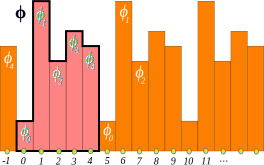
\includegraphics[width=\textwidth]{1dLatStatC_5_0}
\\
{($\shift_1$)}~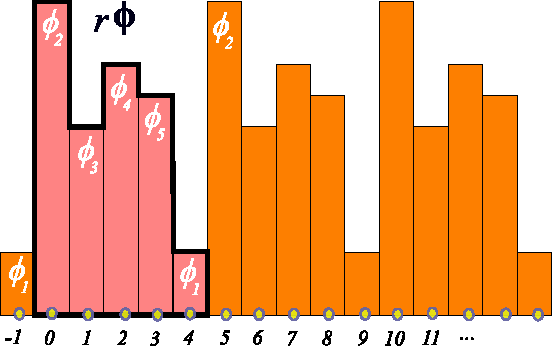
\includegraphics[width=\textwidth]{1dLatStatC_5_1}
\\
{($\shift_2$)}~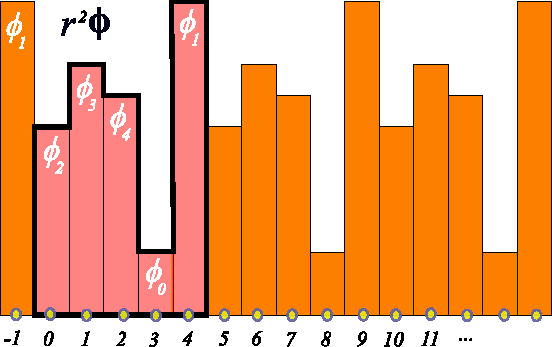
\includegraphics[width=\textwidth]{1dLatStatC_5_2}
\\
{($\shift_3$)}~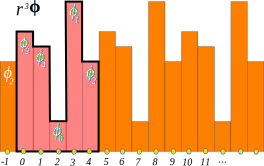
\includegraphics[width=\textwidth]{1dLatStatC_5_3}
\\
{($\shift_4$)}~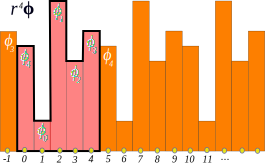
\includegraphics[width=\textwidth]{1dLatStatC_5_4}
  \end{center}\end{minipage}
\qquad\quad
  \begin{minipage}[b]{0.33\textwidth}\begin{center}
{($\Refl$)}~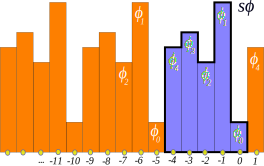
\includegraphics[width=\textwidth]{1dLatStatC_5_s0}
\\
{($\Refl_1$)}~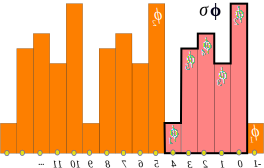
\includegraphics[width=\textwidth]{1dLatStatC_5_s1}
\\
{($\Refl_2$)}~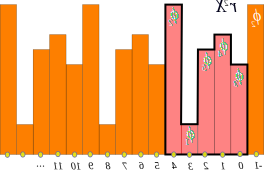
\includegraphics[width=\textwidth]{1dLatStatC_5_s2}
\\
{($\Refl_3$)}~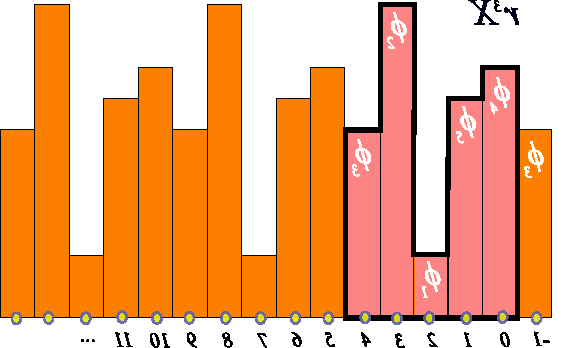
\includegraphics[width=\textwidth]{1dLatStatC_5_s3}
\\
{($\Refl_4$)}~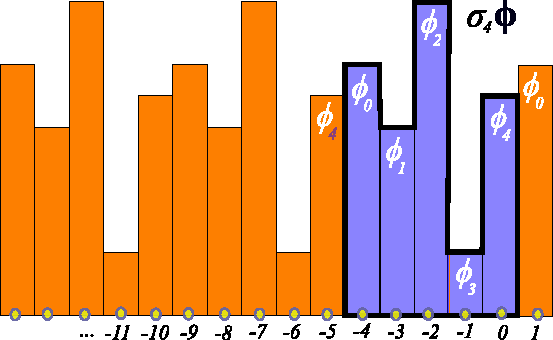
\includegraphics[width=\textwidth]{1dLatStatC_5_s4}

  \end{center} \end{minipage}
  \end{center}
  \caption{\label{fig:1dLatStatC_5}
(Color online)~~~
%Horizontal circles: \lattice\ lattice sites labelled by $\zeit\in\integers$.
%Vertical: the value of field $\ssp_\zeit$, plotted as a bar centred at
%lattice site $\zeit$.
(1)
A Bravais cell $\mathbf{a}$ with
{\lattstate}
% \refeq{1dLattStatC_n}
\(\Xx=\cycle{\ssp_0 \ssp_1 \ssp_2 \ssp_3 \ssp_4}\)
with no reflection symmetry, outlined in bold, invariant under the
translation group $H_{5}$.
Its \Cn{\infty} orbit are the $\cl{}=5$ distinct {\lattstate}s (1) to
($\shift_4$), obtained by all of the $\Cn{5}$ translations.
Its \Dn{\infty}-orbit are $2\cl{}=10$ distinct {\lattstate}s,
5 translations (1) to ($\shift_4$)
and
5 translate-reflections ($\Refl$) to ($\Refl_4$), obtained by
all of the $\Dn{5}$ actions.
See \reffig{LC21FieldConfig}\,(b) for the notation.
Continued in \reffig{fig:symmLattStates}.
          }
\end{figure}
%%%%%%%%%%%%%%%%%%%%%%%%%%%%%%%%%%%%%%%%%%%%%%%%%%%%%

Given that $\Group$ is the {symmetry} of the system does not mean that
$\Group$ is also the symmetry of its solutions, or what we here call {\em
\lattstate}s.
They can satisfy
all of system's symmetries, a subgroup of them, or have no symmetry at
all.
For example, a generic {\lattstate} \refeq{1dLattStat} sketched in
\reffig{fig:HL1dLattRefl} has no symmetry beyond the identity, so its
symmetry group is the trivial subgroup $\{e\}$; any translation
$\shift_j$ or reflection $\Refl_k$ maps it into a different, distinct
{\lattstate}, as shown in \reffig{fig:1dLatStatC_5}.
At the other extreme, the constant {\lattstate}
$\ssp_j=\ssp$ is invariant under any translation or reflections - its
symmetry group is the full \Group, the symmetry of the system. In
between, there are {\lattstate}s whose symmetry is any subgroup of
$\Group$.

%%%%%%%%%%%%%%%%%%%%%%%%%%%%%%%%%%%%%%%%%%%%%%%%%%%%%%%%
\subsection{What are `{\lattstate}s'? Orbits?}
\label{s:LattStates}

Remember, for evolution-in-time, every period-\cl{}\ periodic point is a
fixed point of the \cl{}th iterate of the 1 time-step map. In the lattice
formulation, the totality of finite-period {\lattstate}s is the \emph{set
of fixed points} of all  $H_{\mathbf{a}}$ and  $H_{\mathbf{a},k}$
subgroups of $\Dn{\infty}$.

You can visualize a {\lattstate} invariant under ("fixed by') subgroup
$H_{\mathbf{a},k}$ as a tiling of the lattice $\integers$ by a
{\lattstate} tile of length \cl{}, symmetric under reflection $\Refl_k$,
see \reffig{fig:symmLattStates}\,(b-c).

    \begin{quote}
Definition: {\em
{\em Orbit} or \emph{$\Group$-orbit} of a {\lattstate} $\Xx$ is the
set of all {\lattstate}s
\beq
    \pS_\Xx = \{\LieEl\,\Xx \mid \LieEl \in {\Group}\}
\ee{GroupOrbDisc}
into which $\Xx$ is mapped under the action of group $\Group$.
We label the orbit $\pS_\Xx$ by any {\lattstate} $\Xx$ belonging to
it.
            }
    \end{quote}
As an example, the $\Dn{\infty}$ orbit of the period-5 {\lattstate}
% \refeq{1dLattStatC_n}
% \(\cycle{\ssp_0 \ssp_1 \ssp_2 \ssp_3 \ssp_4}\)
is shown in \reffig{fig:1dLatStatC_5}.
    \PC{2021-09-05} {
    This "maximal subgroup" does not seem to me to be defined here.
    Clean up!
    }
    \begin{quote}
Definition: Symmetry of a solution.
{\em
We shall refer to the maximal subgroup $\Group_\Xx \subseteq  \Group$ of
actions on {\lattstate}s within the orbit $\pS_\Xx$, which leave
the orbit invariant, as the \emph{symmetry}
$\Group_\Xx$ of the orbit $\pS_\Xx$,
\beq
\Group_\Xx =
   \{ \LieEl \in \Group_\Xx \mid \LieEl \Xx \in \pS_\Xx
   %,\,    \LieEl \ssp \neq \ssp  \mbox{ for } \LieEl \neq e
   \}
\,.
\ee{LC21:stabilSet}
}
    \end{quote}
An orbit $\pS_\Xx$ is $\Group_\Xx$-{\em symmetric}
({\em symmetric}, {\em set-wise symmetric}, {\em self-dual})
if the action of elements of $\Group_\Xx$ on
the set of {\lattstate}s $\pS_\Xx$ reproduces the orbit.
%
% \item[2021-07-28 Predrag]
% Rather than Lind's nebulous `index'\rf{Lind96}, for $|\Group/{H}|$ in
% \refeq{Ryu17eq:1.3}
    \begin{quote}
Definition: Multiplicity
{\em
of orbit $\pS_\Xx$ is given by
}
\beq
m_\Xx=|\Group|/|\Group_{\Xx}|
\,.
\ee{GroupOrbMult}
    \end{quote}
(See \toChaosBook{section*.166} {p.~166}.)



\bigskip

And now, a pleasant surprise, obvious upon an inspection of
\reffigs{fig:1dLatStatC_5}{fig:symmLattStates}: what happens
in the Bravais cell, stays in the Bravais cell.
Even though
the lattices \lattice, $\lattice_{\mathbf{a}}$ are infinite,
and their symmetries
$\Dn{\infty}$, $H_{\mathbf{a}}$, $H_{\mathbf{a},k}$ are
\emph{infinite} groups, the Bravais {\lattstate}s'
\emph{orbits} are \emph{finite}, described by the finite group
permutations of the infinite lattice curled up in a Bravais cell periodic
$\cl{}$-site ring.


%\subsection{Finite groups}
%\label{s:1dmnFntPer}


%%%%%%%%%%%%%%%%%%%%%%%%%%%%%%%%%%%%%%%%%%%%%%%%%%%%%%%%%%%%%%%%%%
% PC 2021-08-05:  from ChaosBook book/figs/D3.tex, D3.tex
\begin{figure} \begin{center}
  \begin{minipage}[b]{0.32\textwidth}\begin{center}
  \setlength{\unitlength}{1.00\textwidth}
  \begin{picture}(1,1.12469246)%
    \setlength\tabcolsep{0pt}%
    \put(0,0){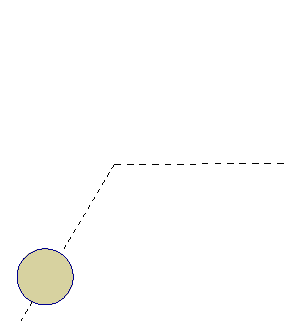
\includegraphics[width=\unitlength,page=1]{D3}}%
    \put(0.23496893,0.6474626){\color[rgb]{0.1372549,0.12156863,0.1254902}\makebox(0,0)[lt]{\smash{$\shift$}}}%
    \put(0,0){\includegraphics[width=\unitlength,page=2]{D3}}%
    \put(0.34167143,0.39068967){\color[rgb]{0.1372549,0.12156863,0.1254902}\makebox(0,0)[lt]{\smash{$\shift_2$}}}%
    \put(0.05464421,0.6373038){\color[rgb]{0.1372549,0.12156863,0.1254902}\makebox(0,0)[lt]{\smash{$\Refl$}}}%
    \put(0.67969793,0.84532127){\color[rgb]{0.1372549,0.12156863,0.1254902}\makebox(0,0)[lt]{\smash{$\Refl_1$}}}%
    \put(0.44996833,0.19132446){\color[rgb]{0.1372549,0.12156863,0.1254902}\makebox(0,0)[lt]{\smash{$\Refl_2$}}}%
    \put(0,0){\includegraphics[width=\unitlength,page=3]{D3}}%
    \put(0.6357866,0.31003627){\color[rgb]{0,0,0}\makebox(0,0)[lt]{\smash{$\pSRed$}}}%
    \put(0.81616715,0.52920775){\color[rgb]{1,1,1}\makebox(0,0)[lt]{\smash{{\Large 0}}}}%
    \put(0.12429459,0.92867118){\color[rgb]{1,1,1}\makebox(0,0)[lt]{\smash{{\Large 1}}}}%
    \put(0.12402384,0.13559257){\color[rgb]{1,1,1}\makebox(0,0)[lt]{\smash{{\Large 2}}}}%
    \put(0,0){\includegraphics[width=\unitlength,page=4]{D3}}%
  \end{picture} \\ $(o)$
  \end{center}\end{minipage}
\qquad
  \begin{minipage}[b]{0.39\textwidth}\begin{center}
  \setlength{\unitlength}{1.00\textwidth}
  \begin{picture}(1,0.94270725)%
    \setlength\tabcolsep{0pt}%
    \put(0,0){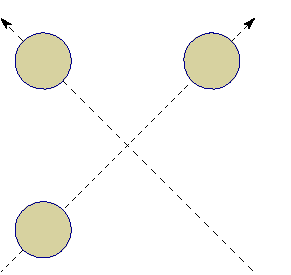
\includegraphics[width=\unitlength,page=1]{D4}}%
    \put(0.11589164,0.70318699){\color[rgb]{1,1,1}\makebox(0,0)[lt]{\smash{{\Large 2}}}}%
    \put(0.11465857,0.11853823){\color[rgb]{1,1,1}\makebox(0,0)[lt]{\smash{{\Large 3
    }}}}%
    \put(0,0){\includegraphics[width=\unitlength,page=2]{D4}}%
    \put(0.69662672,0.11848457){\color[rgb]{1,1,1}\makebox(0,0)[lt]{\smash{{\Large 0}}}}%
    \put(0.69785979,0.70163221){\color[rgb]{1,1,1}\makebox(0,0)[lt]{\smash{{\Large 1}}}}%
    \put(0.48887673,0.58974203){\color[rgb]{0.1372549,0.12156863,0.1254902}\makebox(0,0)[lt]{\smash{$\shift_1$}}}%
    \put(0,0){\includegraphics[width=\unitlength,page=3]{D4}}%
    \put(0.24073374,0.49925981){\color[rgb]{0.1372549,0.12156863,0.1254902}\makebox(0,0)[lt]{\smash{$\shift_2$}}}%
    \put(0.33991763,0.28480816){\color[rgb]{0.1372549,0.12156863,0.1254902}\makebox(0,0)[lt]{\smash{$\shift_3$}}}%
    \put(0.95378545,0.34914366){\color[rgb]{0.1372549,0.12156863,0.1254902}\makebox(0,0)[lt]{\smash{$\Refl_1$}}}%
    \put(0.87112523,0.73973783){\color[rgb]{0.1372549,0.12156863,0.1254902}\makebox(0,0)[lt]{\smash{$\Refl_2$}}}%
    \put(0.50562029,0.87631462){\color[rgb]{0.1372549,0.12156863,0.1254902}\makebox(0,0)[lt]{\smash{$\Refl_3$}}}%
    \put(0.11826698,0.87765494){\color[rgb]{0.1372549,0.12156863,0.1254902}\makebox(0,0)[lt]{\smash{$\Refl$}}}%
    \put(0,0){\includegraphics[width=\unitlength,page=4]{D4}}%
  \end{picture}  \\ $(e)$
  \end{center} \end{minipage}
  \end{center}
  \caption{\label{fig:D3D4}
% Dihedral group \Dn{3}: \Dn{4}:
Translational and rotational symmetries of
    $(o)$
an equilateral triangle,  $\cl{}=3$ lattice sites;
    $(e)$
a square,                  $\cl{}=4$ lattice sites.
The $\cl{}$ rotations $\shift_j$ and the $\cl{}$ translate-reflect
$\Refl_k$ (elements of dihedral group \Dn{\cl{}} \refeq{DnElements},
even reflection axes dashed, odd reflections full line)
overly an $\cl{}$-sided regular polygon onto itself. They
also tile it with  the $2\cl{}$ copies $\pSRed_\ell$ of the fundamental
domain, indicated by the shaded wedge.
}
\end{figure}
%%%%%%%%%%%%%%%%%%%%%%%%%%%%%%%%%%%%%%%%%%%%%%%%%%%%%%%%%%%%%%%

Indeed, to grasp everything one needs to know about translations
$\shift_j$ (for regular polygons, `rotations'),
and
reflections $\Refl_k$,
it suffices to understand the symmetries of
an equilateral triangle (dihedral group \Dn{3})
and
a square (dihedral group \Dn{4}), depicted in \reffig{fig:D3D4}.
It is clear by inspection that an $\cl{}$-sided regular polygon has
$\cl{}$-fold translational symmetry and $\cl{}$ reflection symmetry axes.
The group of such symmetries is the finite dihedral group
\beq
\Dn{\cl{}} = \{1,\Refl,\shift,\Refl_{1},\shift_{2},\Refl_{2},\
           \cdots,
           \shift_{\cl{}-1},\Refl_{\cl{}-1}\}
%\,,
\ee{DnElements}
of order $2\cl{}$.
A half of its elements are the $\cl{}$ cyclic group \Cn{n} translations
$\shift_{j}$.
% 2\pi/n,2\cdot2\pi/n,\cdots$,
The other half are the $\cl{}$ reflections $\Refl_k$, one for the
reflection across each symmetry axis.
The group multiplication table is the same as the $\Dn{\infty}$
\refeq{eq:DinftyMultTab}, but with all subscripts mod $\cl{}$.
%
As in \refeq{DinftyInversion},
conjugation by any reflection reverses the direction of translation
\beq
   \Refl_i\shift_j\Refl_{-i} =  \shift_{\cl{}-j}
\,,\qquad 0<j<\cl{}
\,,
\ee{D_nInversion}now mod $\cl{}$,
so every translation pairs up with the equal counter-translation to form
a 2-element class \refeq{DinftyClassShift}. %$\{\shift_j,\shift_{\cl{}-j}\}$.

The distinction between the classes of even and odd reflections
\refeq{DinftyClassRefl} is visually self-evident by inspection of
\reffig{fig:D3D4}:
the symmetry axes either connect opposite lattice sites, or bisect the
edges, or both, if $\cl{}$ is odd (a triangle, for example).
One can say that the index $k$ in the
`translate-reflection' \refeq{Refl_k} operation
\(
\Refl_{k} %=\Refl\shift_k\,.
\) advances the reflection point by $k$ 1/2 steps, and then reflects
across it.

For a polygon with an \emph{odd} number of
lattice sites (a triangle, for example), we see by contemplating the
triangle of \reffig{fig:D3D4},  as well as by taking  mod $\cl{}$ of the
conjugation relation \refeq{D_nConj}, that
% for  $\cl{}$ odd, the
all reflections are in the same conjugacy class $\{\Refl_{j}\}$:
 there is no splitting into odd and even cases, in
contrast to the infinite lattice case \refeq{DinftyClassRefl}.

For a polygon with an \emph{even} number of lattice sites (a square, for
example), one must distinguish
the `long' axes that connect lattice sites (we label them by even numbers
$0,2,\cdots$)
from
the `short' symmetry axes that bisect opposite edges (labelled by odd
numbers $1,3,\cdots$).
%
The corresponding reflections belong to
different \Dn{\cl{}} (subclasses of
\refeq{DinftyClassRefl},
\bea
\mbox{even reflections}
    &&\quad
\{\Refl,\Refl_{2},\Refl_{4},\cdots,\Refl_{\cl{}/2}\}
    \continue
\mbox{odd reflections}
    &&\quad
\{\Refl_{1},\Refl_{3},\cdots,\Refl_{\cl{}/2+1}\}
\,.
\label{DnClassRefl}
\eea

%%%%%%%%%%%%%%%%%%%%%%%%%%%%%%%%%%%%%%%%%%%%%%%%%%%%%%%%
\subsection{Symmetries of {\lattstate}s}
\label{s:LattStateSyms}


%%%%%%%%%%%%%%%%%%%%%%%%%%%%%%%%%%%%%%%%%%%%%%%%%%%%%
\begin{figure}
  \centering
{$(n)$}
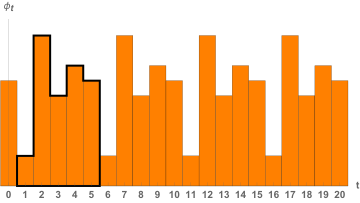
\includegraphics[width=0.40\textwidth]{HL1dLatticeStateBar1}\quad
{$(o)$}
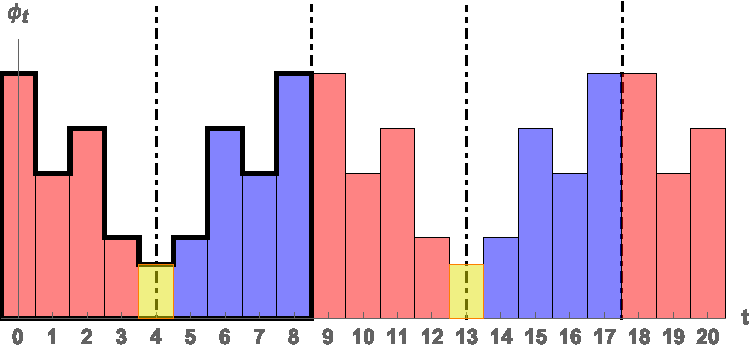
\includegraphics[width=0.40\textwidth]{HL1dLatticeStateBar2}
\\ %~~~
{$(ee)$}
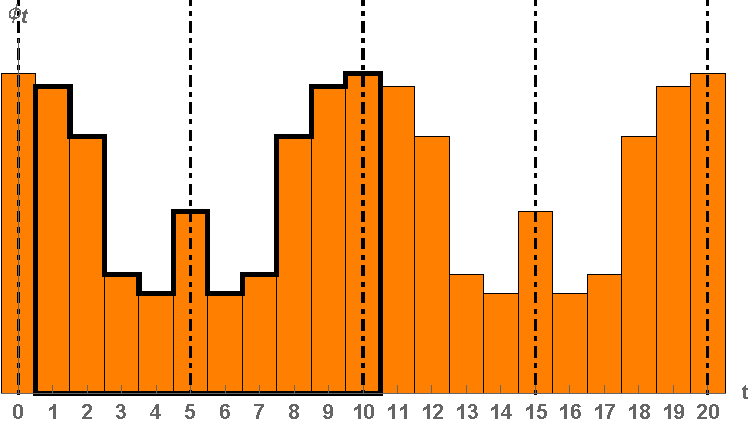
\includegraphics[width=0.40\textwidth]{HL1dLatticeStateBar4}\quad
{$(eo)$}
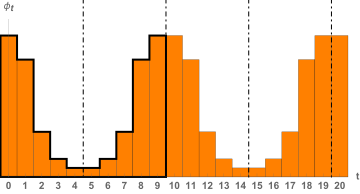
\includegraphics[width=0.40\textwidth]{HL1dLatticeStateBar3}

  \caption{\label{fig:symmLattStates}
(Color online)~~~
A Bravais {\lattstate} \Xx\ has one of the
4 possible symmetries, illustrated by:
$(n)$ {\em No reflection symmetry:}
    an $H_{5}$ invariant period-5 {\lattstate} \refeq{reflSymNo}. For its
    \Group-orbit, see \reffig{fig:1dLatStatC_5}.
$(o)$ {\em Odd period, reflection-symmetric:}
    an $H_{9,8}$ invariant period-9 {\lattstate} \refeq{reflSymOdd},
    %PC 2021-08-21 checked
    reflection symmetric over the lattice sites interval [8-9]  midpoint
    and over the lattice site~4.
$(ee)$ {\em Even period, even reflection-symmetric:}
    an $H_{10,0}$  invariant period-10 {\lattstate} \refeq{reflSymEvens0},
    reflection symmetric over lattice sites 0 and 5.
$(eo)$ {\em Even period, odd reflection-symmetric:}
    an $H_{10,9}$  invariant period-10 {\lattstate} \refeq{reflSymEvens1},
    reflection symmetric over the [4-5] and [9-10] interval midpoints.
Horizontal: lattice sites labelled by $\zeit\in\integers$.
Vertical: value of field $\ssp_\zeit$, plotted as a bar centred at
lattice site $\zeit$.
Even reflection axes dashed, odd reflections full line.
          }
\end{figure}
%%%%%%%%%%%%%%%%%%%%%%%%%%%%%%%%%%%%%%%%%%%%%%%%%%%%%

A Bravais {\lattstate} \Xx\ has one of the
four symmetries:

\bea
    && \mbox{ no reflection symmetry }
    \continue
(n) \quad &&
\cycle{\ssp_0 \ssp_1 \ssp_2 \ssp_3 \cdots \ssp_{\cl{}-1}}
\label{reflSymNo} \\ % the same as {1dLattStatC_n}
    &&
\mbox{ multiplicity } m_\Xx=2\cl{}
    \nnu %\,,
\eea
{\lattstate} invariant under the translation group
$H_{\cl{}}$.
Its \Group-orbit, generated by all actions of \Dn{\infty},
results  in  $2\cl{}$ distinct,  \Dn{\cl{}} related {\lattstate}s.
This is illustrated by the $H_{5}$-invariant {\lattstate} \Xx\ of
\reffig{fig:1dLatStatC_5}. %{fig:symmLattStates}\,$(n)$.
Its \Dn{5} orbit are $2\cl{}=10$ {\lattstate}s, 5  translations
and 5 translate-reflections.
    \PC{2021-08-20} {
    Merge \reffig{fig:symmLattStates}\,$(n)$ with
    \emph{1dLatStatC\_5\_0x3.svg}.
    }

Next, the reflection-symmetric {\lattstate}s.
As illustrated in \reffigs{fig:HL1dLattRefl}{fig:D3D4},
there are two classes \refeq{DinftyClassRefl} of {\lattstate} reflections:
even, across a lattice site, and
odd, across the mid-point between a pair of adjacent lattice sites.
However, as is evident by inspection of \reffig{fig:D3D4}, curling up the
lattice {\lattice} into a Bravais cell periodic $\cl{}$-site ring
implies that an axis cuts the ring twice, and
constrains the possible reflection points to three configurations:

\bea
    && \mbox{ odd period } \cl{}=2m+1
    \continue
(o) \quad &&
\cycle{\sitebox{\ssp_0} \ssp_1 \ssp_2 \cdots \ssp_{m}|\ssp_{m}\cdots \ssp_2 \ssp_1}
\label{reflSymOdd} \\
    &&
\mbox{ multiplicity } m_\Xx=\cl{}
    \nnu %\,,
\eea
{\lattstate} invariant under the dihedral group $H_{\cl{},k}$,
illustrated by the $H_{9,8}$ invariant {\lattstate} \Xx\
of \reffig{fig:symmLattStates}\,$(o)$.
% as well as by the triangle of \reffig{fig:D3D4}\,(1)).
    \PC{2021-08-17} {See \refeq{PCreflSymOdd}.
    We also MUST explain the relation to literature, as
    in the post including \refeq{PC:Ryu17eq:2.11}.
    }
\bea
    && \mbox{ even period } \cl{}=2m+2\,, \mbox{ even reflection } k
    \continue
(ee) \quad &&
\cycle{\sitebox{\ssp_0} \ssp_1 \ssp_2 \cdots \ssp_{m}
        \sitebox{\ssp_{m+1}} \ssp_{m} \cdots \ssp_2 \ssp_1}
\label{reflSymEvens0} \\
    &&
\mbox{ multiplicity } m_\Xx=\cl{}/2
    \nnu %\,,
\eea
{\lattstate} invariant under the dihedral group $H_{\cl{},k}$,
$k$ even,
illustrated by the $H_{10,0}$ invariant {\lattstate} \Xx\
of \reffig{fig:symmLattStates}\,$(ee)$.
\bea
    && \mbox{ even period } \cl{}=2m\,, \mbox{ odd reflection } k
    \continue
(eo) \quad &&
\cycle{\ssp_1 \ssp_2 \ssp_3 \cdots \ssp_{m}| \ssp_{m}\cdots \ssp_2 \ssp_1|}
\label{reflSymEvens1} \\
    &&
\mbox{ multiplicity } m_\Xx=\cl{}/2
    \nnu %\,,
\eea
{\lattstate} invariant under the dihedral group $H_{\cl{},k}$,
$k$ odd,
illustrated by the $H_{10,9}$ invariant {\lattstate} \Xx\
of \reffig{fig:symmLattStates}\,$(eo)$.

For long periods $\cl{}$, almost all orbits are of no-symmetry type
\refeq{reflSymNo}.
So why do we care about the symmetric orbits so much? The reason is that
the \po\ expansions are dominated by the short orbits, and many, if not
the most of those are reflection-symmetric.

The {\lattstate} {symmetry} $\Group_\Xx$ \refeq{LC21:stabilSet} of the
above $(o)$--$(eo)$ reflection-symmetric {\lattstate}s \Xx\ is the reflection
group $\Dn{1}=\{1,\Refl_k\}$, but we will spare the reader the
group-theorist's cosets and group quotients. For us, this symmetry means
two things:
\begin{itemize}
  \item[(1)]
The \Dn{\infty} orbits of reflection-symmetric {\lattstate}s contain only
translations, as any reflection amounts to a cyclic group
\Cn{\cl{}} translation.
(Try reflecting a  {\lattstate} in \reffig{fig:symmLattStates}\,(b-d)
over any lattice site or mid-interval.)
  \item[(2)]
{\lattstate} is a `half' of it, the length ${m}$ orbit,
\beq
\tilde{\Xx}      = \ssp_1 \ssp_2 \ssp_3 \cdots \ssp_{m}
\,.
\ee{primeLattStat}


\end{itemize}
Reflection breaks the translational invariance, and how one reconstructs
the period-$\cl{}$ orbit from this length-$m$ \brick\ is a bit tricky. To
develop intuition about that, it is helpful to have a look at a matrix
representation of $\Dn{\cl{}}$.

%%%%%%%%%%%%%%%%%%%%%%%%%%%%%%%%%%%%%%%%%%%%%%%%%%%%%%%%%%%%%%%%%%%%%%%%%%
\section{Permutation representation}
\label{sect:permReps}

A {\lattstate} {\Xx} over a Bravais cell $\mathbf{a}$ can be assembled
into an $\cl{}$\dmn\ vector whose components are lattice site fields
\beq
\transp{\Xx} = (\ssp_0,\ssp_1,\ssp_2,\ssp_3,\cdots,\ssp_{\cl{}-1})
\,,
\ee{1dLattStatVec}
with the first field in such vector placed at the lattice site 0, the
second at the lattice site 1, and so on. Matrices that reshuffle the
components of such vectors form the {\em permutation representation} of a
finite group \Group, which gives us a different and helpful
perspective on the three kinds of symmetric solutions of the preceding
section.

The permutation representation of 1-step lattice translation $\shift$
acts on a Bravais {\lattstate} by the off-diagonal
$[\cl{}\!\times\!\cl{}]$ matrix \refeq{hopMatrix}. This is a cyclic
\Cn{\cl{}} permutation that translates the {\lattstate} $\Xx$
"forward-in-time" by one site,
\[
\transp{(\shift\Xx)}=(\ssp_1,\ssp_2,\cdots,\ssp_{\cl{}-1},\ssp_0)
\,.
\]
A permutation representation of a \Dn{\cl{}} translate-reflect should
morally be an anti-diagonal matrix that reverses the order of site
fields,
\[
\transp{(\Refl_k\Xx)}=(\ssp_{\cl{}-1},\cdots,\ssp_2,\ssp_1,\ssp_0)
\,.
\]
Symmetries of triangles and squares help us make this precise.

%     \item[2021-03-09 Han]
\emph{Odd period}:
In odd dimensions, the $\cl{}$ translate-reflect matrices of \Dn{\cl{}} are
related by translations \refeq{D_nConj}.

A period-3 example: For $\cl{}=3$ {\lattstate}
with out symmetry
\(
\transp{\Xx} = (\ssp_0,\ssp_1,\ssp_2)
\,,
\)
they are
\[
\Refl=
\left(
\begin{array}{ccc}
 1 & 0 & 0 \\
 0 & 0 & 1 \\
 0 & 1 & 0
\end{array}
\right)
    \,,\quad
{\Refl_1}=
\left(
\begin{array}{ccc}
 0 & 1 & 0 \\
 1 & 0 & 0 \\
 0 & 0 & 1
\end{array}
\right)
    \,,\quad
\Refl_2=
\left(
\begin{array}{ccc}
 0 & 0 & 1 \\
 0 & 1 & 0 \\
 1 & 0 & 0
\end{array}
\right)
\,.
\]
In agreement with \refeq{reflSymOdd}, \reffig{fig:D3D4}\,$(o)$ and
\reffig{fig:symmLattStates}\,$(o)$, reflections keep one lattice site fixed
(for each permutation matrix $\Refl_k$ there is only one `1' on the
diagonal), swap the rest.

A period-5 example: reflection symmetric {\lattstate}s tiles the infinite lattice
\lattice\ with a reflection-fixed $\sitebox{\ssp_0}$, and a length-2
{\brick} $(\ssp_1,\ssp_2)$,
\beq
\Xx =
\cdots \ssp_2 \ssp_1 \sitebox{\ssp_0} \ssp_1 \ssp_2 |
      \ssp_2 \ssp_1 \sitebox{\ssp_0} \ssp_1 \ssp_2 |\cdots
\,.
\ee{symmCycD5}
\Dn{5} permutation representation of reflections of a pentagon, illustrates that
fixpoints {\Xx} of $\Refl_{k}$ are cyclicly related:
\bea
\Refl\Xx &=&
\left(
\begin{array}{ccccc}
 1 & 0 & 0 & 0 & 0 \\
 0 & 0 & 0 & 0 & 1 \\
 0 & 0 & 0 & 1 & 0 \\
 0 & 0 & 1 & 0 & 0 \\
 0 & 1 & 0 & 0 & 0
\end{array}
\right)
\left(\begin{array}{c}
 \sitebox{\ssp_0}\cr
 \ssp_1\cr
 \ssp_2\cr
 \ssp_2\cr
 \ssp_1\cr
\end{array}\right)
=
\left(\begin{array}{c}
 \sitebox{\ssp_0}\cr
 \ssp_1\cr
 \ssp_2\cr
 \ssp_2\cr
 \ssp_1\cr
\end{array}\right)
        \continue
\Refl_{4}(\shift_{-2}\Xx )
     &=&
\left(
\begin{array}{ccccc}
 0 & 0 & 0 & 0 & 1 \\
 0 & 0 & 0 & 1 & 0 \\
 0 & 0 & 1 & 0 & 0 \\
 0 & 1 & 0 & 0 & 0\\
 1 & 0 & 0 & 0 & 0
\end{array}
\right)
\left(\begin{array}{c}
 \ssp_2\cr
 \ssp_1\cr
 \sitebox{\ssp_0}\cr
 \ssp_1\cr
 \ssp_2\cr
\end{array}\right)
=
\left(\begin{array}{c}
 \ssp_2\cr
 \ssp_1\cr
 \sitebox{\ssp_0}\cr
 \ssp_1\cr
 \ssp_2\cr
\end{array}\right)
\,.
\label{symmCycD5Refl}
\eea

The symmetry conditions are the Bravais lattice site 5-periodicity
mod 5, and the even reflection across
$\sitebox{\ssp_0}$:
\beq
\ssp_{i} = \ssp_{i+5}
    \,, \quad
\ssp_{-i} = \ssp_{i}
\,.
\ee{symmCycD5bcs}
A {\lattstate} satisfies
the defining equation \refeq{LC21:1dTempFT} %{catMapNewt}
\beq
- \ssp_{\zeit-1}  +  V'(\ssp_{\zeit}) - \ssp_{\zeit+1}
    =
\Ssym{\zeit}
\,,
\ee{LC21:1dTempFTa} %{catMapHL}
on the period-5 Bravais cell,
\bea
    V'(\ssp_{0}) - 2 \ssp_1 &=& m_0 \continue
-\ssp_0 +V'(\ssp_{1}) -\ssp_2 &=& m_1 \continue
-\ssp_1 +V'(\ssp_{2}) -\ssp_2 &=& m_2 \continue
-\ssp_1 +V'(\ssp_{2}) -\ssp_2 &=& m_2 \continue
-\ssp_0 +V'(\ssp_{1}) -\ssp_2 &=& m_1
\label{symmCycD5eqs5} % from {HLsymmCycD5eqs}
\eea
where we have used \refeq{symmCycD5bcs}.
The result is a length-3 \brick\ {\lattstate} condition for
$\sitebox{\ssp_0}$, followed by the 2-{\brick} $(\ssp_1,\ssp_2)$,
\bea
    V'(\ssp_{0}) - 2 \ssp_1 &=& m_0 \continue
-\ssp_0 +V'(\ssp_{1}) -\ssp_2 &=& m_1 \continue
-\ssp_1 +V'(\ssp_{2}) -\ssp_2 &=& m_2
\label{symmCycD5eqs} % from {HLsymmCycD5eqs}
\eea
with a 3\dmn\ {\jacobianOrb} \refeq{jMorb1dFT}
\bea
\jMorb_+ &=&
\left(\begin{array}{ccc}
{s}_0 & -2 & 0 \\
 -1 & {s}_1 & -1 \\
 0 & -1 & {s}_2-1
\end{array}\right)
\,,
\label{OrbJacobianD5} % from {HLOrbJacobianD5}
\eea

While the translational symmetry is broken, the even
$\sitebox{\ssp_0}$ and odd $|$ reflection \bcs\ only affect the
top and the bottom rows.

The {\jacobianOrb} \refeq{jMorb1dFT}, 3 symmetry cases:


\emph{Odd period} Bravais cell \refeq{reflSymOdd},
is $[(m+1)\times(m+1)]$\dmn\
(compare with \refeq{HLreflectionSymOdd}):
        \PC{2021-09-01} {
The bottom, odd, looks like Neumann boundary condition, see
Pozrikidis\rf{Pozrikidis14} \CBlibrary{Pozrikidis14} eq.~(1.5.4).
The top, time-direction symmetry breaking b.c. I do not recognize.
    }
\beq
\jMorb[\Xx] =
\left(\begin{array}{cccccccc}
%\begin{pmatrix}
{s}_{0} & {\color{red}-2} & 0 & 0 & \cdots & 0 & 0 & {\color{red}0} \\
-1 & {s}_{1} & -1 & 0 & \cdots & 0 & 0 & 0 \\
0 & -1 & {s}_{2} & -1 & \cdots & 0 & 0 & 0 \\
\vdots & \vdots & \vdots & \vdots & \ddots & \vdots & \vdots & \vdots \\
0 & 0 & 0 & 0 & \cdots & -1 & {s}_{m-1} & -1 \\
{\color{red}0} & 0 & 0 & 0 & \cdots & 0 & -1 & {s}_{m} {\color{red}-1}
%\end{pmatrix}
          \end{array} \right)
\,.
\ee{jMorb1dFTodd}

\emph{Even period} $\cl{}=2m+2$, \emph{even reflection} $k$ \refeq{reflSymEvens0}
(compare with \refeq{HLreflectionSymSecondKind}):
\beq
\jMorb[\Xx] =
\left(\begin{array}{cccccccc}
%\begin{pmatrix}
{s}_{0} & {\color{red}-2} & 0 & 0 & \cdots & 0 & 0 & {\color{red}0} \\
-1 & {s}_{1} & -1 & 0 & \cdots & 0 & 0 & 0 \\
0 & -1 & {s}_{2} & -1 & \cdots & 0 & 0 & 0 \\
\vdots & \vdots & \vdots & \vdots & \ddots & \vdots & \vdots & \vdots \\
0 & 0 & 0 & 0 & \cdots & -1 & {s}_{m} & -1 \\
{\color{red}0} & 0 & 0 & 0 & \cdots & 0 &  {\color{red}-2} & {s}_{m+1}
%\end{pmatrix}
          \end{array} \right)
\,.
\ee{jMorb1dFTEvens0}

\emph{Even period} $\cl{}=2m$, \emph{odd reflection}  $k$ \refeq{reflSymEvens1}
(compare with \refeq{HLreflectionSymFirstKind}):
\beq
\jMorb[\Xx] =
\left(\begin{array}{ccccccc}
%\begin{pmatrix}
 {s}_{1} {\color{red}-1}& -1 & 0 & \cdots & 0 & 0 & {\color{red}0} \\
 -1 & {s}_{2} & -1 & \cdots & 0 & 0 & 0 \\
 \vdots & \vdots & \vdots & \ddots & \vdots & \vdots & \vdots \\
 0 & 0 & 0 & \cdots & -1 & {s}_{m-1} & -1 \\
{\color{red}0} & 0 & 0 & \cdots & 0 & -1 & {s}_{m} {\color{red}-1}
%\end{pmatrix}
          \end{array} \right)
\,.
\ee{jMorb1dFTEvens1}


\bigskip\bigskip

 {\jacobianOrb} $\jMorb$ evaluated on the {\lattstate}
 commutes with $\Refl$,
\beq
\jMorb\Refl%  = \shift - s\id + \shift^{-1}
  =
\left(\begin{array}{ccccc}
 {s}_0& -1 & 0 & 0 & -1 \\
 -1 &  {s}_1& -1 & 0 &0\\
 0 & -1 &  {s}_2& -1 &0 \\
 0 & 0 & -1 & {s}_2& -1 \\
 -1 & 0 & 0 & -1 &  {s}_1
\end{array} \right)
\left(
\begin{array}{ccccc}
 1 & 0 & 0 & 0 & 0 \\
 0 & 0 & 0 & 0 & 1 \\
 0 & 0 & 0 & 1 & 0 \\
 0 & 0 & 1 & 0 & 0 \\
 0 & 1 & 0 & 0 & 0
\end{array}
\right)
=\Refl \jMorb
\,.
\ee{LC21Hessian}


\bigskip\bigskip

\emph{Even period} examples:
For even dimensions, there are two classes of reflections,
the even ones, \reffig{fig:symmLattStates}\,$(ee)$, that leave two `yellow'
site fields fixed, swap the rest,
and
the odd ones, \reffig{fig:symmLattStates}\,$(eo)$, that swap the
`reds' and `blues'.
This is illustrated by the \Dn{4} permutation representation of the  even
$\Refl$, odd $\Refl_{3}$ reflection symmetries of a square,
\reffig{fig:D3D4}\,$(e)$:
\beq
\Refl =
\left(
\begin{array}{cccc}
 1 & 0 & 0 & 0 \\
 0 & 0 & 0 & 1 \\
 0 & 0 & 1 & 0 \\
 0 & 1 & 0 & 0
\end{array}
\right)
    \,,\quad
\Refl_{3} =
\left(
\begin{array}{cccc}
 0 & 0 & 0 & 1 \\
 0 & 0 & 1 & 0 \\
 0 & 1 & 0 & 0 \\
 1 & 0 & 0 & 0
\end{array}
\right)
\,.
\ee{D4Refl03}
The even reflection keeps two site fields fixed,
\[
\transp{(\Refl\Xx)}=(\sitebox{\ssp_{0}},\ssp_3,\sitebox{\ssp_2},\ssp_1)
\,,
\]
in agreement with \refeq{reflSymEvens0}.
while
 the odd reflection reverses the order of site fields
\[
\transp{(\Refl_{3}\Xx)}=(\ssp_{3},\ssp_2|\ssp_1,\ssp_0)
\,,
\]
in agreement with \refeq{reflSymEvens1},


\bigskip\bigskip\bigskip

\refeq{HLsymmCycD8s1}
is invariant under the 1/2 lattice spacing reflection:
\bea
\Refl=
\left(
\begin{array}{ccccccccc}
 0 & 0 & 0 & 0 & 0 & 0 & 0 & 1 \\
 0 & 0 & 0 & 0 & 0 & 0 & 1 & 0 \\
 0 & 0 & 0 & 0 & 0 & 1 & 0 & 0 \\
 0 & 0 & 0 & 0 & 1 & 0 & 0 & 0 \\
 0 & 0 & 0 & 1 & 0 & 0 & 0 & 0 \\
 0 & 0 & 1 & 0 & 0 & 0 & 0 & 0 \\
 0 & 1 & 0 & 0 & 0 & 0 & 0 & 0 \\
 1 & 0 & 0 & 0 & 0 & 0 & 0 & 0 \\
\end{array}
\right)
\,.
\eea

\refeq{HLsymmCycD8s0}
the corresponding
reflection operator leaves sites 1 and 4 invariant:
\bea
\Refl_1=
\left(
\begin{array}{ccccccccc}
 1 & 0 & 0 & 0 & 0 & 0 & 0 & 0 \\
 0 & 0 & 0 & 0 & 0 & 0 & 0 & 1 \\
 0 & 0 & 0 & 0 & 0 & 0 & 1 & 0 \\
 0 & 0 & 0 & 0 & 0 & 1 & 0 & 0 \\
 0 & 0 & 0 & 0 & 1 & 0 & 0 & 0 \\
 0 & 0 & 0 & 1 & 0 & 0 & 0 & 0 \\
 0 & 0 & 1 & 0 & 0 & 0 & 0 & 0 \\
 0 & 1 & 0 & 0 & 0 & 0 & 0 & 0 \\
\end{array}
\right)
\,.
%\label{HL-ReflD9-1}
\eea


Combination $\shift+\shift^{-1}$
%in \refeq{SVWorbitJac}
commutes with $\Refl_k$,
and $\Refl_k$ conjugacy reverses ${\mathbb{S}}$
\bea
\Refl_k\jMorb\Refl_k &=&-\shift+\Refl_k{\mathbb{S}}\,\Refl_k-\shift^{-1}
    \continue
            &=&
\left(\begin{array}{ccccccc} %\begin{bmatrix}
{s}_{n-1} & -1 & 0 & 0 & \dots & 0 & -1\\
-1 & {s}_{n-2} & -1 & 0 & \dots & 0 & 0\\
0 & -1 & {s}_2 & -1 & \dots & 0 & 0\\
\vdots & \vdots & \vdots & \vdots & \ddots & \vdots & \vdots\\
0 & 0 & \dots & \dots & \dots & {s}_{2} & -1\\
-1 & 0 & \dots & \dots & \dots & -1 & {s}_{1}
\end{array}\right) %\end{bmatrix}
%\label{LC21:reverOrbitJac}
\eea
where ${\mathbb{S}}$ is a diagonal matrix with the lattice site $k$ `stretching'
factor ${s}_k$ in the $k$th row/column.

If a period-9 orbit is invariant under the reflection operator (see
\refeq{HL-ReflD9-1})
\bea
\Refl=
\left(
\begin{array}{ccccccccc}
 0 & 0 & 0 & 0 & 0 & 0 & 0 & 0 & 1 \\
 0 & 0 & 0 & 0 & 0 & 0 & 0 & 1 & 0 \\
 0 & 0 & 0 & 0 & 0 & 0 & 1 & 0 & 0 \\
 0 & 0 & 0 & 0 & 0 & 1 & 0 & 0 & 0 \\
 0 & 0 & 0 & 0 & 1 & 0 & 0 & 0 & 0 \\
 0 & 0 & 0 & 1 & 0 & 0 & 0 & 0 & 0 \\
 0 & 0 & 1 & 0 & 0 & 0 & 0 & 0 & 0 \\
 0 & 1 & 0 & 0 & 0 & 0 & 0 & 0 & 0 \\
 1 & 0 & 0 & 0 & 0 & 0 & 0 & 0 & 0 \\
\end{array}
\right)
\,.
%\label{ReflD9-0}
\eea

If a period-8 orbit is of form (see \refeq{reflSymEvens0}) %{HLsymmCycD8s0})
\beq
\cycle{\sitebox{\ssp_0} \ssp_1 \ssp_2 \ssp_3 \sitebox{\ssp_4} \ssp_3 \ssp_2 \ssp_1}
\,,
\eeq %\ee{symmCycD8s0}
the corresponding
reflection operator leaves sites 0 and 4 invariant  (see \refeq{HL-ReflD9-1}):
\bea
\Refl=
\left(
\begin{array}{ccccccccc}
 1 & 0 & 0 & 0 & 0 & 0 & 0 & 0 \\
 0 & 0 & 0 & 0 & 0 & 0 & 0 & 1 \\
 0 & 0 & 0 & 0 & 0 & 0 & 1 & 0 \\
 0 & 0 & 0 & 0 & 0 & 1 & 0 & 0 \\
 0 & 0 & 0 & 0 & 1 & 0 & 0 & 0 \\
 0 & 0 & 0 & 1 & 0 & 0 & 0 & 0 \\
 0 & 0 & 1 & 0 & 0 & 0 & 0 & 0 \\
 0 & 1 & 0 & 0 & 0 & 0 & 0 & 0 \\
\end{array}
\right)
\,.
%\label{ReflD9-1}
\eea

%%%%%%%%%%%%%%%%%%%%%%%%%%%%%%%%%%%%%%%%%%%%%%%%%%%%%%%%%%%%%%
\begin{table} %[ht]
\caption{\label{tab:LC21HenCycD5} % extracted from {tab:orbitdet}
    The {\henlatt} period-5 and -6 symmetric {\lattstate}s of type
    \reffig{fig:symmLattStates}\,(b), with symmetry indicated in the
    $\Refl$-reflection format \refeq{symmCycD5Refl}. %{HLsymmCycD5}.
    For odd $\cl{}=2m+1$, symmetric orbits reduce to {\brick}s of length $m+1$.
    For even $\cl{}=2m$, their lengths are either $m+1$ or $m$.
    The period-5 {\lattstate}s are plotted in \reffig{fig:PChenlatt5cyc}
    (to supersede \reffig{SVW5CycHamHen}\,(left)).
    There is no asymmetric period-5, the first $\Cn{\cl{}}$ asymmetric pair is
    period-6.
    Indicated: the binary code $\Ssym{j}$ of the field $\ssp_j$
    at the lattice site $j=0,1,2,3,4$.
         }
\centering
\begin{tabular}{|lll|} % right alligned columns (2 columns)
%\hline\hline %inserts double horizontal lines
\hline
 \Cn{5}  & $\ssp_{-2} \ssp_{-1} \sitebox{\ssp_0}\,\ssp_1 \ssp_2 |$ & \Dn{5}
\\[0.5ex]
 $11110$ & $11\,\sitebox{0}\,11\,|$ & $\sitebox{0}\,11\,|$\\
 $00011$ & $10\,\sitebox{0}\,01\,|$ & $\sitebox{0}\,01\,|$\\
 $00101$ & $01\,\sitebox{0}\,10\,|$ & $\sitebox{0}\,10\,|$\\
 $00001$ & $00\,\sitebox{1}\,00\,|$ & $\sitebox{1}\,00\,|$\\[0.5ex]
 $11010$ & $10\,\sitebox{1}\,01\,|$ & $\sitebox{1}\,01\,|$\\
 $11100$ & $01\,\sitebox{1}\,10\,|$ & $\sitebox{1}\,10\,|$\\
[1ex]
\hline
\end{tabular}
~~~~
\begin{tabular}{|lll|} % next table
\hline
 \Cn{6}  & $\ssp_0 \ssp_1 \ssp_2 \ssp_3 \ssp_4 \ssp_5$ & \Dn{6}
\\ [0.5ex]
 $001011$ & $001011$ & $001011$\\
 $110100$ & $110100$ &  \\
\hline
 & $\sitebox{\ssp_0} \ssp_1 \ssp_2 \sitebox{\ssp_3} \ssp_2 \ssp_1$ &
\\ [0.5ex]
 $010001$ & $\sitebox{0}\,10\,\sitebox{0}\,01$ & $\sitebox{0}\,10\,\sitebox{0}$\\
 $011111$ & $\sitebox{0}\,11\,\sitebox{1}\,11$ & $\sitebox{0}\,11\,\sitebox{1}$\\
 $001110$ & $\sitebox{0}\,01\,\sitebox{1}\,10$ & $\sitebox{0}\,01\,\sitebox{1}$\\
 $100000$ & $\sitebox{1}\,00\,\sitebox{0}\,00$ & $\sitebox{1}\,00\,\sitebox{0}$\\
 $101110$ & $\sitebox{1}\,01\,\sitebox{1}\,10$ & $\sitebox{1}\,01\,\sitebox{1}$\\
\hline
 & $ \ssp_0  \ssp_1 \ssp_2 | \ssp_2 \ssp_1 \ssp_0|$ &
\\ [0.5ex]
 $001100$ & $001|100|$ & $|001|$\\
 $011110$ & $011|110|$ & $|011|$\\
[1ex]
\hline
\end{tabular}
\end{table}
%%%%%%%%%%%%%%%%%%%%%%%%%%%%%%%%%%%%%%%%%%%%%%%%%%%%%%%%%%%%%%
